%auto-ignore
\documentclass{standalone}

\usepackage{graphicx}
\usepackage{tikz}
\usetikzlibrary{fit}

\begin{document}
\begin{tikzpicture}
\node[inner sep=0pt,label=left:{$i - 1$}]
(fapl1) at (0,10)
	{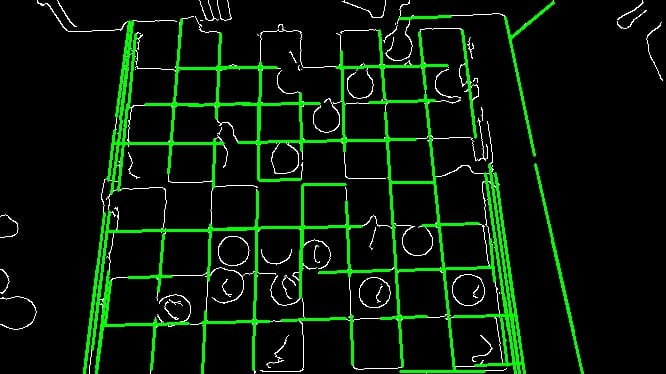
\includegraphics[trim=0 325 0
	0,clip,keepaspectratio,width=1.5\textwidth]{figure4_i1.jpg}};
\node[inner sep=0pt,label=left:{$i$}]
(fapl2) at (0,8)
	{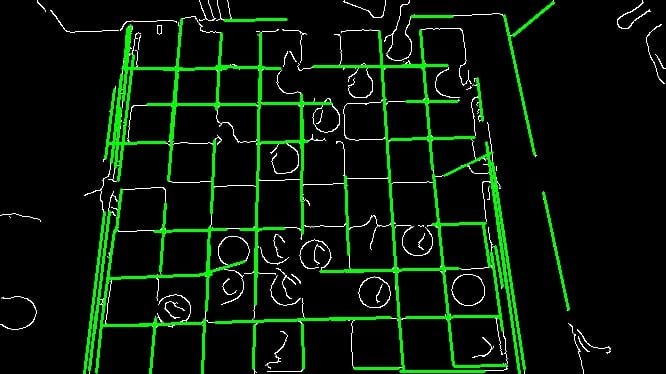
\includegraphics[trim=0 325 0
	0,clip,keepaspectratio,width=1.5\textwidth]{figure4_i2.jpg}};
\node[inner sep=0pt,label=left:{$i + 1$}]
(fapl3) at (0,6)
	{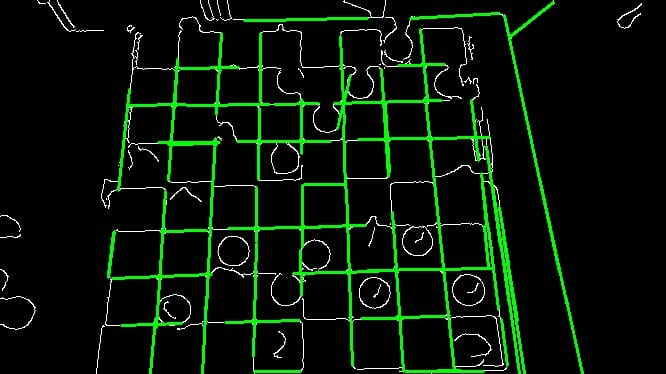
\includegraphics[trim=0 325 0
	0,clip,keepaspectratio,width=1.5\textwidth]{figure4_i3.jpg}};
\node[inner sep=0pt,label=left:{\textbf{analysis}}]
(fapl_all) at (0,4)
	{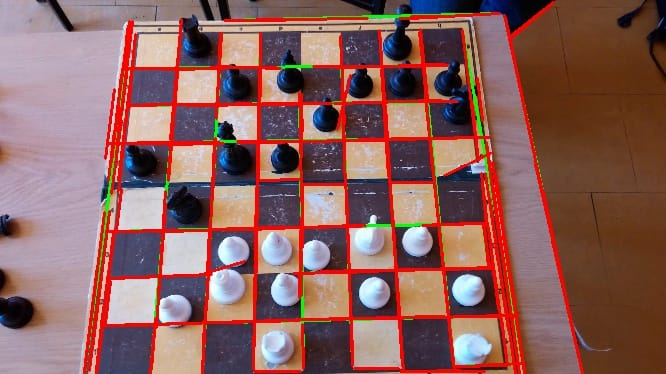
\includegraphics[trim=0 325 0
	0,clip,keepaspectratio,width=1.5\textwidth]{figure4_a.jpg}};
\node[inner sep=0pt,label=left:{\textbf{final}}]
(fapl_lines) at (0,2)
	{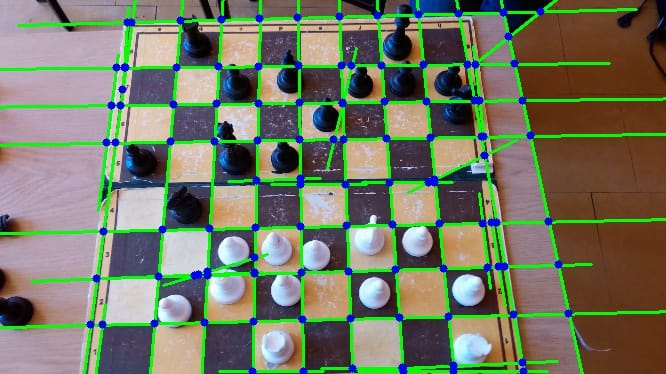
\includegraphics[trim=0 325 0
	0,clip,keepaspectratio,width=1.5\textwidth]{figure4_b.jpg}};
\node[left=1.5em,inner xsep=1.5em,draw,dotted,fit=(fapl1) (fapl2) (fapl3)] {};
\end{tikzpicture}
\end{document}
